
\chapter{Discrete Random Variables}


\section{The Notion of a Random Variable}

\bit
	\item The outcome of a random experiment \emph{need not be a number}.
	However, we are usually interested not in the outcome itself,
	but rather in \emph{some measurement or numerical attribute} of the outcome.

	\item A \emph{random variable} $X$ is a function
	that assigns a real number, $X(\zeta)$,
	to each outcome $\zeta$ in the sample space of a random experiment.
	(\lgfig{3.1})

	\item The sample space \sspace\ is the \emph{domain} of the random variable,
	and the set \ssx\ of all values taken on by \X\ is the \emph{range} of the random variable.

	\item Capital letters denote \randvar s, \eg, \X\ or $Y$,
	and lower case letters denote possible values of the \randvar s,
	\eg, $x$ or $y$

	\item \lgexam{3.1}{Coin Tosses}

	\item For random variables,
	the function or rule that assigns values to each outcome is \emph{fixed and deterministic}.
	Therefore the distribution of the values of a random variable \X\ is
	determined by the probabilities of the outcomes \mzeta\ in the random experiment.
	In other words, the randomness in the observed values of \X\ is
	induced by the \emph{underlying random experiment}.
	\[
		\pr{X \in B} = \pr{ \set{\zeta}{X(\zeta)\in B}}
	\]

\eit

\section{Discrete Random Variables and Probability Mass Function}

\bit
	\item A \emph{discrete random variable \X}
	is defined as a random variable that assumes values from a \emph{countable set},
	that is, $\ssx = \{x_1, x_2, x_3, \ldots \}$.
	A discrete random variable is said to be \emph{finite} if its range is finite,
	that is, $\ssx = \xcomma{x}{n}$.

	\item We \emph{only need to obtain the probabilities for the events
	$A_k = \set{\zeta}{X(\zeta)=x_k}$}.


	\item The probability mass function (PMF)
	of a discrete random variable \X\ is defined as:
	\beql{eq-def-pmf}
		\pmfxk{x_k} = \pr{X=x_k} = \pr{A_k}
		\mfor x\in\reals.
	\eeql

	\item The events \xcommai{A}\ form a \emph{partition} of \sspace\
	as illustrated in \lgfig{3.3}.
	\begin{proof}
	\begin{itemize}
		\item For $j\neq k$,
		\[
			A_j \cap A_k = \set{\zeta}{X(\zeta) = x_j \mand X(\zeta) = x_k}
			= \emptyset
		\]
		since $X(\zeta)$ cannot have two different values; it's a function.

		\item For each $\zeta\in\sspace$, $X(\zeta)=x_k$ for some $k$ since \xcommai{x}\
		is a range of the function $X(\zeta)$.
		Hence
		\[
			\sspace = \bigcupktoi A_k.
		\]
	\end{itemize}
	\end{proof}

	\item
	The PMF \pmfxk{x}\ satisfies three properties
	that provide all the information required to calculate probabilities
	for events involving the discrete random variable $X$:
	\begin{enumerate}
		\item Axiom I implies
		\beql{eq-pmf-prop-1}
			\pmfxk{x} = \pr{\set{\zeta}{X(\zeta)=x}}\geq 0 ~\forall x.
		\eeql

		\item Axiom II implies
		\beql{eq-pmf-prop-2}
			\sum_{x\in\ssx} \pmfxk{x}
			= \sum_{x\in\ssx} \pr{\set{\zeta}{X(\zeta) = x}}
			= \sumktoi \pr{A_k}
			= \pr{\sspace} = 1.
		\eeql

		\item Axiom III' implies
		\beql{eq-pmf-prop-3}
			\pr{X\in B}
			= \bpr{\bigcup_{x\in B} \set{\zeta}{X(\zeta) = x}}
			= \bpr{\bigcup_{x_k\in B}{A_k}}
			= \sum_{x_k \in B} \pr{A_k}
			= \sum_{x_k \in B} \pmfxk{x_k}.
		\eeql
	\end{enumerate}


	\item
	The PMF of \X\ gives us the probabilities for \emph{all the elementary events} from \ssx.

	\item
	If we are only interested in events concerning \X,
	then we can forget about the underlying random experiment
	and its associated probability law
	and \emph{just work with \ssx\ and the PMF of \X}.

	\item \lgexam{3.5}{Coin Tosses and Binomial Random Variable}

	\item \lgfig{3.4(a)} and \lgfig{3.4(b)}
	show the graph of \pmfxk{x}\ versus $x$
	for the random variables.
	In general, the graph of the PMF
	of a discrete random variable has \emph{vertical arrows} of height \pmfxk{x_k}\
	at the values $x_k$ in \ssx.

	\item The \emph{uniform \randvar}: $\pmfxk{k} = 1/M$ for $k\in\{1,2,\ldots,M\}$.

	\item
	The \emph{Bernoulli random variable} $\indi{A}$ is equal to $1$
	if $A$ occurs and zero otherwise,
	and is given by the indicator function for $A$:
	\[
		\indi{A}(\zeta) = \left\{ \begin{array}{ll}
			1	&\mif \zeta\in A,
			\\0	&\mif \zeta \notin A.
		\end{array}
		\right.
	\]
	If $\pr{A}=p$,
	\beql{eq-bern-pmf}
		\pmf{I}(x) = \left\{ \begin{array}{ll}
			\pr{\set{\zeta}{\zeta\in\comp{A}}} = p	&\mif x = 1
			\\\pr{\set{\zeta}{\zeta\in A}}= 1-p	&\mif x=0.
		\end{array}
		\right.
	\eeql

	\item \lgexam{3.9}{Message Transmission}
	$X$ is a discrete random variable taking
	on values from $\ssx = \{1, 2, 3, \ldots\}$.
	The event $\{X = k\}$ occurs if the underlying experiment
	finds $k - 1$ consecutive erroneous transmissions
	(``failures'')
	followed by an error-free one (``success''):
	\beql{eq-geo-pmf}
		\pmfxk{k} = (1-p)^{k-1} p
		\mfor k=1,2,\ldots
	\eeql

	We call \X\ the \emph{geometric random variable},
	and we say that \X\ is \emph{geometrically distributed}.

	\item \lgexam{3.10}{Transmission Errors}
	A binary communications channel introduces
	a bit error in a transmission with probability $p$.
	Let \X\ be the number of errors in $n$ independent transmissions.
	Find the PMF of \X.
	Find the probability of one or fewer errors.

	\beql{eq-binom-pmf}
		\pmfxk{k} = \pr{X=k} = {n \choose{k}} p^k(1-p)^{n-k}
		\mfor k=1,2,\ldots
	\eeql
	We call \X\ the \emph{binomial random variable}.

	\item The graph of relative frequencies should approach the graph of the PMF.
	(\lgfig{3.5})

	\item \emph{the relationship between relative frequencies and the PMF \pmfxk{x_k}}.
	Suppose we perform \emph{$n$ independent repetitions}
	to obtain $n$ observations of the discrete random variable \X.
	Let $N_k(n)$ be the number of times the event
	$X = x_k$ occurs and let
	$f_k(n) = N_k(n)/n$
	be the corresponding relative frequency.
	As $n$ becomes large we expect that $f_k(n) \to \pmfxk{x_k}$.
	Therefore \emph{the graph of relative frequencies should approach
	the graph of the PMF}.
	(\lgfig{3.5(a)})
\eit

\section{Expected Value and Moments of Discrete Random Variable}
\bit
	\item
	In some situations
	we are interested in a few parameters
	that summarize the information provided by the PMF.
	(\lgfig{3.6})

	\item
	The \emph{expected value} or \emph{mean}
	of a discrete random variable \X\ is defined by
	\beql{eq-def-expect}
		\expect{X} = \Expect {X}
		= \sum_{x\in\ssx} x \pmfxk{x}
		= \sum_k x_k \pmfxk{x_k}.
	\eeql
	The expected value $\Expect{X}$ is defined if the above sum converges absolutely,
	that is,
	\beql{eq-abs-sum}
		\Expect{|X|} = \sum_k |x_k| \pmfxk{x} < \infty.
	\eeql

	\item If we view \pmfxk{x}\
	as the distribution of mass on the points \xcommai{x}\ in the real line,
	then \Expect{X} represents the \emph{center of mass of this distributiona}.

	\item \lgexam{3.11}{Mean of Bernoulli Random Variable}
	\[
		\Expect{I_A} = 0 \pmf{I}(0) + 1 \pmf{I}(1) = p.
	\]

	\item
	The use of the term ``expected value''
	\emph{does not mean that we expect to observe \Expect{X}}
	when we perform the experiment that generates \X.

	\item The arithmetic average, or \emph{sample mean}, of the observations,
	is
	\begin{eqnarray}
		\lefteqn
		{
			\samplemean{X}{n}
			= \frac{x(1)+x(2)+\cdots+x(n)}{n}
			= \frac{x_1N_1(n) + x_2N_2(n) + \cdots}{n}
		}
		\nonumber
		\\&=& x_1f_1(x) + x_2f_2(x) + \cdots
		= \sum_k x_k f_k(n).
		\label{eq-sample-mean}
	\end{eqnarray}
	As $n$ becomes large,
	we expect relative frequencies to approach the probabilities \pmfxk{x_k}:
	\[
		\lim_{n\to\infty} f_k(n) \to \pmfxk{x_k} \mforall k,
	\]
	hence
	\[
		\samplemean{X}{n} = \sum_k x_k f_k(n)
		\to \sum_k x_k \pmfxk{x_k} = \Expect{X}.
	\]

	\item \lgexam{3.15}{Mean of a Geometric Random Variable}
	Let \X\ be the number of bytes in a message,
	and suppose that \X\ has a geometric distribution with parameter $p$.
	Find the mean of \X.

	By definition,
	\[
		\Exp{X} = \sumktoi k p q^{k-1},
	\]
	thus (\ref{eq-is-kxk-2}) implies
	\[
		\Exp{X} = p \sumktoi k q^{k-1} = p/(1-q)^2 = 1/p.
	\]

	\item \lgexam{3.16}{St. Petersburg Paradox}
	A fair coin is tossed repeatedly until a tail comes up.
	If \X\ tosses are needed,
	then the casino pays the gambler $Y = 2^X$
	dollars.
	How much should the gambler be willing to pay to play this game?

	\begin{itemize}
		\item Random variables with \emph{unbounded expected value}
		are not uncommon and appear in models where outcomes that have extremely large values
		are not that rare.
		Examples include the sizes of files in
		\emph{Web transfers, frequencies of words in large bodies of text,
		and various financial and economic problems}.
	\end{itemize}

	\item Expected value is a \emph{linear operator}:
	Assume two random variables $X$ and $Y$
	and two real numbers $a$ and $b$. Then
	\beql{eq-exp-lin-operator}
		\Exp{aX+bY} = a\Exp{X} + b\Exp{Y}.
	\eeql

\eit

\subsection{Expected Value of Functions of a Random Variable}
\bit
	\item Let \X\ be a discrete random variable,
	and let $Z = g(X)$.
	Since \X\ is discrete,
	$Z = g(X)$ will assume a \emph{countable set of values}
	of the form $g(x_k)$ where $x_k \in \ssx$.
	Denote the set of values assumed by $g(X)$
	by $\{\xcommai{z}\}$.
	One way to find the expected value of $Z$
	is to use (\ref{eq-def-expect}),
	which requires that we first find the PMF of $Z$.
	\beql{eq-expect-z}
		\Exp{Z} = \sum_j z_j \pmf{Z}(z_j).
	\eeql
	Another way is to use the following result:
	\beql{eq-expect-fcn}
		\Exp{Z} = \Exp{g(X)} = \sum_k g(x_k) \pmfxk{x_k}.
	\eeql

	To show the equivalence of (\ref{eq-expect-z}) and (\ref{eq-expect-fcn}),
	we group the terms $x_k$ that are mapped to each value $z_j$:
	\[
		\sum_k g(x_k) \pmfxk{x_k}
		=  \sum_j z_j \left( \sum_{x_k:g(x_k)=z_j} \pmfxk{x_k} \right)
		= \sum_j z_j \pmf{Z}(z_j) = \Exp{Z}.
	\]

	\item \lgexam{3.17}{Square-Law Device}
	Let \X\ be a noise voltage that is uniformly distributed
	in $\ssx = \{-3, -1, +1, +3\}$
	with $\pmfxk{k} = 1/4$ for $k$ in \ssx.
	Find \Exp{Z}\  where $Z = X^2$.

\eit


\subsection{Variance of a Random Variable}
\bit
	\item
	We are interested not only in the mean of a random variable,
	but also in the \emph{extent of the random variable's variation} about its mean.

	\newcommand{\mx}{\expect{X}}
	\item The \emph{variance of the random variable \X}
	is defined as the expected value of the square of the deviation about the mean,
	$(X-\Exp{X})^2$:

	\beql{eq-def-var}
		\std{X}^2 = \VAR{X} = \Exp{(X-\expect{X})^2}
		= \sum_{x\in\ssx} (x-\expect{X})^2 \pmfxk{x}
		= \sum_k (x_k-\expect{X})^2 \pmfxk{x_k}.
	\eeql

	An alternative expression for the variance:
	\beql{eq-def-var-2}
		\Exp{(X-\mx)^2}
		 = \Exp{X^2-2 \mx X + \mx^2}
		 = \Exp{X^2}-2 \mx \Exp{X} + \mx^2
		 = \Exp{X^2}-\mx^2
	\eeql

	\item The \emph{$n$th moment of \X} is defined by
	\beql{eq-n-moment-x}
		\Exp{X^n}
	\eeql
	\begin{itemize}
		\item the \emph{second moment of \X} is $\Exp{X^2}$.
	\end{itemize}


	\item The \emph{standard deviation of the random variable \X} is defined
	by the square root of the variance of \X:
	\beql{eq-def-std}
		\std{X} = \STD{X} = \VAR{X}^{1/2}
	\eeql

	\item \emph{Neither} the variance \emph{nor} the standard deviation is a linear operator, but
	\begin{itemize}
		\item \emph{Adding a constant} to a random variable
		does not affect the variance.
		\[
			\VAR{X+c}
			= \Exp{(X+c - (\Exp{X}+c))^2}
			= \Exp{(X - \Exp{X})^2}
			= \VAR{X}.
		\]

		\item \emph{Scaling a random variable} by $c$
		scales the variance by $c^2$ and the standard deviation by $|c|$:
		\[
			\VAR{cX}
			= \Exp{(cX - c\Exp{X})^2}
			= \Exp{c^2(X - \Exp{X})^2}
			= c^2\Exp{(X - \Exp{X})^2}
			= c^2\VAR{X},
		\]
		thus
		\[
			\STD{cX} = |c|~\STD{X}
		\]

	\end{itemize}

	\item \lgexam{3.22}{Variance of Geometric Random Variable}
	Find the mean and \var\ of the \geomrv.

	The infinite series formula (\ref{eq-is-kxk-2}) implies
	\beql{eq-geomrv-mean}
		\Exp{X} = \sumktoi k q^{k-1} p = p / (1-q)^2 = 1/p.
	\eeql
	The second moment of \X\ is
	\beql{eq-geomrv-2-moment}
		\Exp{X^2} = \sumktoi k^2 q^{k-1} p = (1+q)p/(1-q)^3 = (1+q)/p^2
	\eeql
	where (\ref{eq-is-ksxk}) is used,
	thus the \var\ is
	\beql{eq-geomrv-var}
		\VAR{X} = \Exp{X^2} - \expect{X}^2
		= (1+q)/p^2 - 1/p^2 = q/p^2 = (1-p)/p^2.
	\eeql

\eit


\section{Conditional Probability Mass Function}
\subsection{Conditional Probability Mass Function}
\bit
	\item The \emph{conditional probability mass function}
	of \X\ is defined by the conditional probability:
	\beql{eq-def-cond-pmf}
		\cpmfxk{x}{C}
		 = \cpr{X=x}{C}
	\eeql
	or equivalently
	\beql{eq-def-cond-pmf-1}
		\cpmfxk{x}{C}
		 = \cpreq{\{X=x\}}{C}
	\eeql
	The above expression has a nice intuitive interpretation:
	The conditional probability of the event $\{X = x_k\}$
	is given by the probabilities of outcomes $\zeta$
	for which \emph{both $X(\zeta) = x_k$ and $\zeta$ are in $C$,
	normalized by \pr{C}}.

	\item The conditional PMF satisfies
	properties like
	(\ref{eq-pmf-prop-1}), (\ref{eq-pmf-prop-2}), and (\ref{eq-pmf-prop-3}):
	\begin{enumerate}
		\item $ \cpmfxk{x_k}{C} \geq 0$ for all $x_k\in\ssx$.

		\item $ \sum_{x_k\in\ssx} \cpmfxk{x_k}{C} = 1$.

		\item $ \cpr{X\in B}{C}
			= \sum_{x_k \in B} \cpmfxk{x_k}{C} \mbox{ where } B \subset \ssx  $.
	\end{enumerate}
	\begin{proof}
	It is obvious that $\cpmfxk{x_k}{C}\geq0$ for all $x_k \in\ssx$.
	Since the set of the events $A_k = \set{\zeta}{X(\zeta)=x_k}$
	is a partition of \sspace,
	\[
		\sum_{x\in\ssx} \cpmfxk{x}{C}
		= \sum_{x\in\ssx} \cpr{X=x}{C}
		= \sum_{x\in\ssx} \pr{\{X=x\}\cap C} /\pr{C}
		= \pr{C}/\pr{C} = 1.
	\]
	Since $A_k$ are mutually exclusive,
	$A_k \cap C$ are mutually exclusive
	and
	\begin{eqnarray*}
		\lefteqn{
		\pr{\{X\in B\}\cap C}
		= \bpr{\left(\bigcup_{x_k\in B} A_k\right) \cap C}
		}
		\\& =& \bpr{\bigcup_{x_k\in B} (A_k \cap C)}
		= \sum_{x_k \in B} \pr{A_k \cap C}
		= \sum_{x_k \in B} \pr{\{X=x_k\} \cap C}.
	\end{eqnarray*}
	Thus
	\[
		\cpr{X\in B}{C}
		= \cpreq{\{X\in B \}}{C}
		= \sum_{x_k \in B} \frac{\pr{\{X=x_k\} \cap C}}{\pr{C}}
		= \sum_{x_k \in B} \cpmfxk{x_k}{C}.
	\]
	\end{proof}


	\item \lgexam{3.24}{Residual Waiting Times}
	Let \X\ be the time required to transmit a message,
	where \X\ is a uniform random variable with $\ssx = \{1, 2, \ldots, L\}$.
	Suppose that a message has already been transmitting for $m$ time units,
	find the probability that the remaining transmission time is $j$ time units.

	We are given $C = \{X>m\}$, so for $m+1\leq m_j\leq L$,
	\[
		\cpmfxk{m+j}{X>m} = \frac{\pr{X=m+j}}{\pr{X>m}}
		= \frac{1/L}{1-m/L} = \frac{1}{L-m}
	\]
	for $1\leq j\leq L-m$.

	\item
	Let \xcomma{B}{n}\ be a partition for the sample space \sspace.
	The theorem on total probability allows us
	to find the \emph{PMF of \X\ in terms of the conditional PMF's}:
	\beql{eq-pmf-total-prob}
		\pmfxk{x} = \sumiton \cpmfxk{x}{B_i} \pr{B_i}.
	\eeql
	\begin{proof}
		The theorem on total probability implies
		\[
			\pr{A} = \sumkton \cpr{A}{B_k}\pr{B_k}
		\]
		where $A = \set{\zeta}{X(\zeta)=x}$.
	\end{proof}

	\item \lgexam{3.25}{Device Lifetimes}
	A production line yields two types of devices.
	Type $1$ devices occur with probability $\alpha$
	and work for a relatively short time
	that is geometrically distributed with parameter $r$.
	Type $2$ devices work much longer,
	occur with probability $1 - \alpha$,
	and have a lifetime that is geometrically distributed with parameter $s$.
	Let \X\ be the lifetime of an arbitrary device. Find the PMF of \X.

	The conditional probabilities can be found as
	\[
		\cpmfxk{k}{B_1} = (1-r)^{k-1} r \mfor k \in \naturals
	\]
	and
	\[
		\cpmfxk{k}{B_2} = (1-s)^{k-1} s \mfor k \in \naturals.
	\]
	Thus,
	\[ 
		\pmfxk{k} = \cpmfxk{k}{B_1} \pr{B_1} + \cpmfxk{k}{B_2} \pr{B_2}
		= (1-r)^{k-1} r\alpha
		+ (1-s)^{k-1} s(1-\alpha).
	\]
\eit

\subsection{Conditional Expected Value}
\newcommand{\mxb}{\ensuremath{\expect{X|B}}}
\bit
	\item The \emph{conditional expected value of \X\ given $B$} is defined as:
	\beql{eq-def-cond-expect}
		\expect{X|B} = \cExp{X}{B}
		= \sum_{x\in\ssx} x \cpmfxk{x}{B}
		= \sum_k x_k \cpmfxk{x_k}{B}
	\eeql
	where we apply the absolute convergence requirement on the summation

	\item The \emph{conditional variance of \X\ given $B$} is defined as:
	\beql{eq-def-cond-var}
		\cVAR{X}{B}
		= \cExp{(X-\mxb)^2}{B}
		= \sum_k (x_k - \mxb)^2 \cpmfxk{x_k}{B}
		= \cExp{X^2}{B} - \mxb^2
	\eeql
	Note that the variation is \emph{measured with respect to \mxb, not \expect{X}}.

	\item Let \xcomma{B}{n}\ be a partition for the sample space \sspace,
	and let \cpmfxk{x}{B_i}\ be the conditional PMF of \X\ given event $B_i$.
	\emph{\Exp{X}\ can be calculated from the conditional expected values \cExp{X}{B}}:
	\beql{eq-expect-total-prob}
		\Exp{X} = \sumiton \cExp{X}{B_i} \pr{B_i}.
	\eeql
	\begin{proof}
	The theorem on total probability implies
	\begin{eqnarray*}
		\Exp{X} &=& \sum_k x_k \pmfxk{x_k}
		= \sum_k x_k \left( \sumiton \cpmfxk{x_k}{B_i} \pr{B_i} \right)
		= \sumiton \left( \sum_k x_k \cpmfxk{x_k}{B_i} \right) \pr{B_i}
		\\&=& \sumiton \cExp{X}{B_i} \pr{B_i}.
	\end{eqnarray*}
	\end{proof}

	\item Using the same approach we can also show
	\beql{eq-expect-fcn-total-prob}
		\Exp{g(X)} = \sumiton \cExp{g(X)}{B_i} \pr{B_i}.
	\eeql
	\begin{proof}
	The theorem on total probability implies
	\begin{eqnarray*}
		\Exp{g(X)} &=& \sum_k g(x_k) \pmfxk{x_k}
		= \sum_k g(x_k) \left( \sumiton \cpmfxk{x_k}{B_i} \pr{B_i} \right)
		\\&-& \sumiton \left( \sum_k g(x_k) \cpmfxk{x_k}{B_i} \right) \pr{B_i}
		= \sumiton \cExp{g(X)}{B_i} \pr{B_i}.
	\end{eqnarray*}
	\end{proof}

	\item \lgexam{3.26}{Device Lifetimes}
	Find the mean and variance for the devices in \lgexamref{3.25}.

	Note that (\ref{eq-geomrv-mean}) and (\ref{eq-geomrv-2-moment}) imply
	\begin{eqnarray*}
		&\cExp{X}{B_1} = 1/r,&
		\cExp{X^2}{B_1} = (2-r)/r^2,
		\\
		&\cExp{X}{B_2} = 1/s,&
		\cExp{X^2}{B_2} = (2-s)/s^2.
	\end{eqnarray*}
	Now (\ref{eq-expect-total-prob}) and (\ref{eq-expect-fcn-total-prob}) imply that
	\[
		\Exp{X} = \cExp{X}{B_1} \alpha +  \cExp{X}{B_2} (1-\alpha)
		= \alpha/r + (1-\alpha)/s
	\]
	and
	\begin{eqnarray*}
		\lefteqn{
		\VAR{X} = \Exp{X^2} - \expect{X}^2
		}
		\\ &=&
		\cExp{X^2}{B_1} \alpha +  \cExp{X^2}{B_2} (1-\alpha) - \expect{X}^2
		\\ &=&
		\alpha (2-r)/r^2 + (1-\alpha) (2-s)/s^2 - ( \alpha/r + (1-\alpha)/s )^2.
	\end{eqnarray*}
	(I think the author made a mistake on this.)
	\begin{itemize}
		\item Note that we do \emph{not} use the conditional variances
		to find \VAR{Y}\ because (\ref{eq-expect-fcn-total-prob})
		does not apply to (conditional) variances.
		However, the equation \emph{does} apply to the \cond\ second moments.
	\end{itemize}

\eit

\section{Important Discrete Random Variables}
\bit
	\item Certain random variables arise in many diverse,
	unrelated applications.
	The pervasiveness of these random variables
	is due to the fact
	that \emph{they model fundamental mechanisms} that underlie random behavior.

	\item
	\emph{Discrete random variables} arise mostly in applications
	where \emph{counting is involved}.
\eit

\subsection{The Bernoulli Random Variables}
\bit
	\item The Bernoulli random variable $I_A$
	equals one if the event $A$ occurs,
	and zero otherwise.

	\begin{itemize}
		\item range:
		\beql{eq-range-bernoulli}
			\ssx = \{0,1\}.
		\eeql
		\item PMF:
		\beql{eq-pmf-bernoulli}
			p_I(0) = 1-p,\ 
			p_I(1) = p.
		\eeql
		where $\pr{A} = p$.
		\figurename~\ref{fig-bernoulli-pmf} shows the PMF when $p=0.6$.

		\item mean and variance:
		\beql{eq-mean-bernoulli}
			\Expect{X} = p.
		\eeql
		\beql{eq-var-bernoulli}
			\VAR{X} = \Exp{I_A^2} - \Expect{X}^2
			= p - p^2 = pq.
		\eeql
	\end{itemize}
	\begin{figure}\begin{center}
	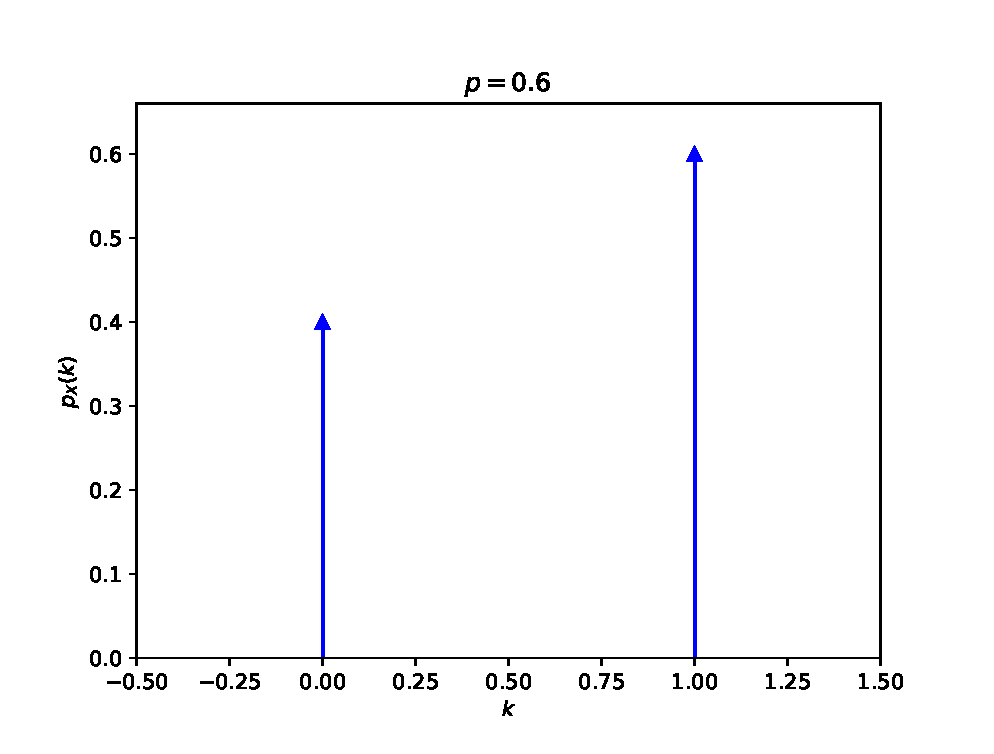
\includegraphics[width=.7\linewidth]{figures/bernoulli_pmf}
	\caption{The PMF of the \bernrv\ with $p=0.6$}
	\label{fig-bernoulli-pmf}
	\end{center}\end{figure}

	\item The maximum variability occurs when $p = 1/2$
	which corresponds to the case that is most difficult to predict.

\eit

\subsection{The Binomial Random Variables}
\bit
	\item The binomial \randvar\ \X\
	is (can be) defined by the number of successes in
	$n$ independent Bernoulli trials.
	\begin{itemize}
		\item range:
		\beql{eq-range-binom}
			\ssx = \{0,1,\ldots, n \}.
		\eeql
		\item PMF:
		\beql{eq-pmf-binom}
			\pmfxk{k} = \chs{n}{k} p^k (1-p)^{n-k}.
		\eeql
		\figurename~\ref{fig-binom-pmf} shows the PMFs of the two \binomrv s;
		one with with $n=5$ and $p=0.3$
		and the other with with $n=10$ and $p=0.6$.

		\item mean and variance:
		\beql{eq-mean-binom}
			\Exp{X} = np.
		\eeql
		\beql{eq-var-binom}
			\VAR{X} = npq.
		\eeql
	\end{itemize}
	
	\begin{figure}\begin{center}
	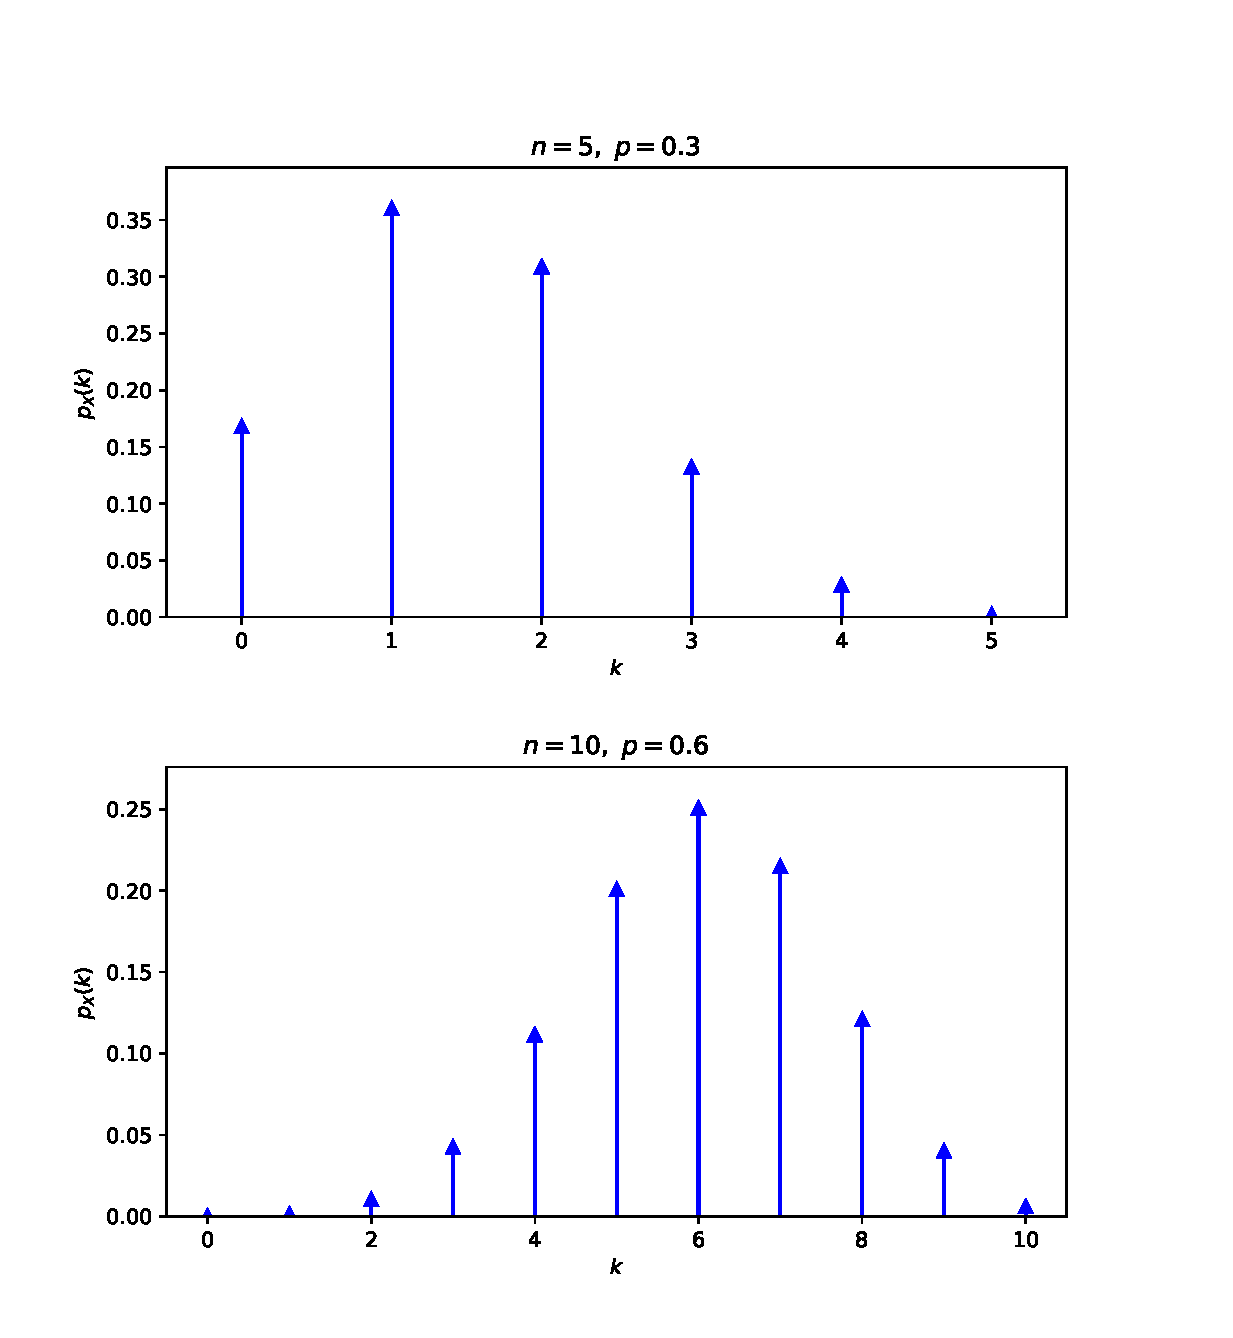
\includegraphics[width=.7\linewidth]{figures/binom_pmf}
	\caption{The PMFs of the two \binomrv s}
	\label{fig-binom-pmf}
	\end{center}\end{figure}

	\begin{proof}
		First, let know check whether the sum of all the PMF values is $1$.
		The binomial theorem in \S\ref{app-math} implies
		\[
			\sumto{k}{0}{n} \pmfxk{k}
			= \sumto{k}{0}{n} \chs{n}{k} p^k (1-p)^{n-k}
			= (p+q)^n =1,
		\]
		hence the proof.
		The expected value can be evalued as
		\begin{eqnarray*}
			\lefteqn{
			\Exp{X} = \sumto{k}{0}{n} k \chs{n}{k} p^k (1-p)^{n-k}
			= \sumto{k}{1}{n} \frac{n!}{(k-1)!(n-k)!} p^k (1-p)^{n-k}
			}
			\\ &=&
			np \sumto{k}{1}{n} \frac{(n-1)!}{(k-1)!(n-k)!} p^{k-1} (1-p)^{n-k}
			\\ &=&
			np \sumto{k}{1}{n} \frac{(n-1)!}{(k-1)!((n-1)-(k-1))!} p^{k-1} (1-p)^{((n-1)-(k-1))}
			\\ &=&
			np \sumto{k}{0}{n-1} \frac{(n-1)!}{k!((n-1)-k)!} p^{k-1} (1-p)^{((n-1)-k)}
			\\ &=&
			np
		\end{eqnarray*}
		where the last equality comes from 
		that the last summation is equal to
		the sum of the PMFs of the \binomrv\ with $n-1$ and $p$.
		The second moment of \X\ is
		\begin{eqnarray*}
			\lefteqn{
			\Exp{X^2} = \sumto{k}{0}{n} k^2 \chs{n}{k} p^k (1-p)^{n-k}
			= \sumto{k}{1}{n} k \frac{n!}{(k-1)!(n-k)!} p^k (1-p)^{n-k}
			}
			\\ &=&
			\sumto{k}{0}{n-1} (k+1) \frac{n!}{(k)!(n-k-1)!} p^{k+1} (1-p)^{n-1-k}
			\\ &=&
			np \sumto{k}{0}{n-1} (k+1) \frac{(n-1)!}{(k)!(n-k-1)!} p^{k} (1-p)^{n-1-k}
			\\ &=&
			np \sumto{k}{0}{n-1} (k+1) \chs{n-1}{k} p^{k} (1-p)^{n-1-k}
			\\ &=&
			np \sumto{k}{0}{n-1} k \chs{n-1}{k} p^{k} (1-p)^{n-1-k}
			+ np \sumto{k}{0}{n-1} \chs{n-1}{k} p^{k} (1-p)^{n-1-k}
			\\ &=&
			n(n-1)p^2 + np
			= n^2p^2 -np^2 + np
			= n^2p^2 +npq,
		\end{eqnarray*}
		thus
		\[
			\VAR{X} = \Exp{X^2} - \Exp{X}^2 = npq.
		\]
		The alternative proofs can be found in \S\ref{app-proofs}.
		\label{loc-binom-alter-proof}
	\end{proof}

	\item The expected value $\Exp{X} = np$
	\emph{agrees with our intuition}
	since we expect a fraction $p$ of the outcomes to result in success.

	\item The variance of the binomial is $n$ times
	the variance of a Bernoulli random variable.
	The variance becomes maximum when $p=1/2$
	for the same reason that the maximum variance of the Bernoulli \randvar\
	is achieved when $p=1/2$.

	\item The maximum PMF occurrs at
	$k_\mathrm{max}= \floor{(n + 1)p}$, where $\floor{x}$
	denotes the largest integer
	that is smaller than or equal to $x$.
	When $(n + 1)p$ is an integer,
	then the maximum is achieved at \kmax\
	and $\kmax + 1$.

	\item The ratio of \pmfxk{k+1}\ and \pmfxk{k}: 
	\[
		\frac{\pmfxk{k+1} }{\pmfxk{k}}
		= {\chs{n}{k+1} p^{k+1} q^{n-k-1} }/ {\chs{n}{k} p^{k} q^{n-k} }
		= \frac{n-k}{k+1} \frac{p}{q}.
	\]
	This can be used for calculation of the PMF of the \binomrv.
	Should this concern us?
\eit

\subsection{The Geometric Random Variable}
\bit
	\item The geometric random variable arises
	when we count the number of independent Bernoulli trials
	until the first occurrence of a success.
	The number $X$ is called the \emph{geometric random variable}
	and it takes on values from the set $\{1, 2, \ldots\}$.

	\begin{itemize}
		\item range:
		\beql{eq-range-geom}
			\ssx = \naturals = \{1,2,\ldots \}.
		\eeql
		\item PMF:
		\beql{eq-pmf-geom}
			\pmfxk{k} = (1-p)^{k-1} p.
		\eeql
		\figurename~\ref{fig-geom-pmf} shows the PMFs of the two \geomrv s;
		one with $p=0.3$
		and the other with $p=0.5$.

		\item mean and variance:
		\beql{eq-mean-geom}
			\Exp{X} = 1/p.
		\eeql
		\beql{eq-var-geom}
			\VAR{X} = (1-p)/p^2.
		\eeql
	\end{itemize}

	\begin{figure}\begin{center}
	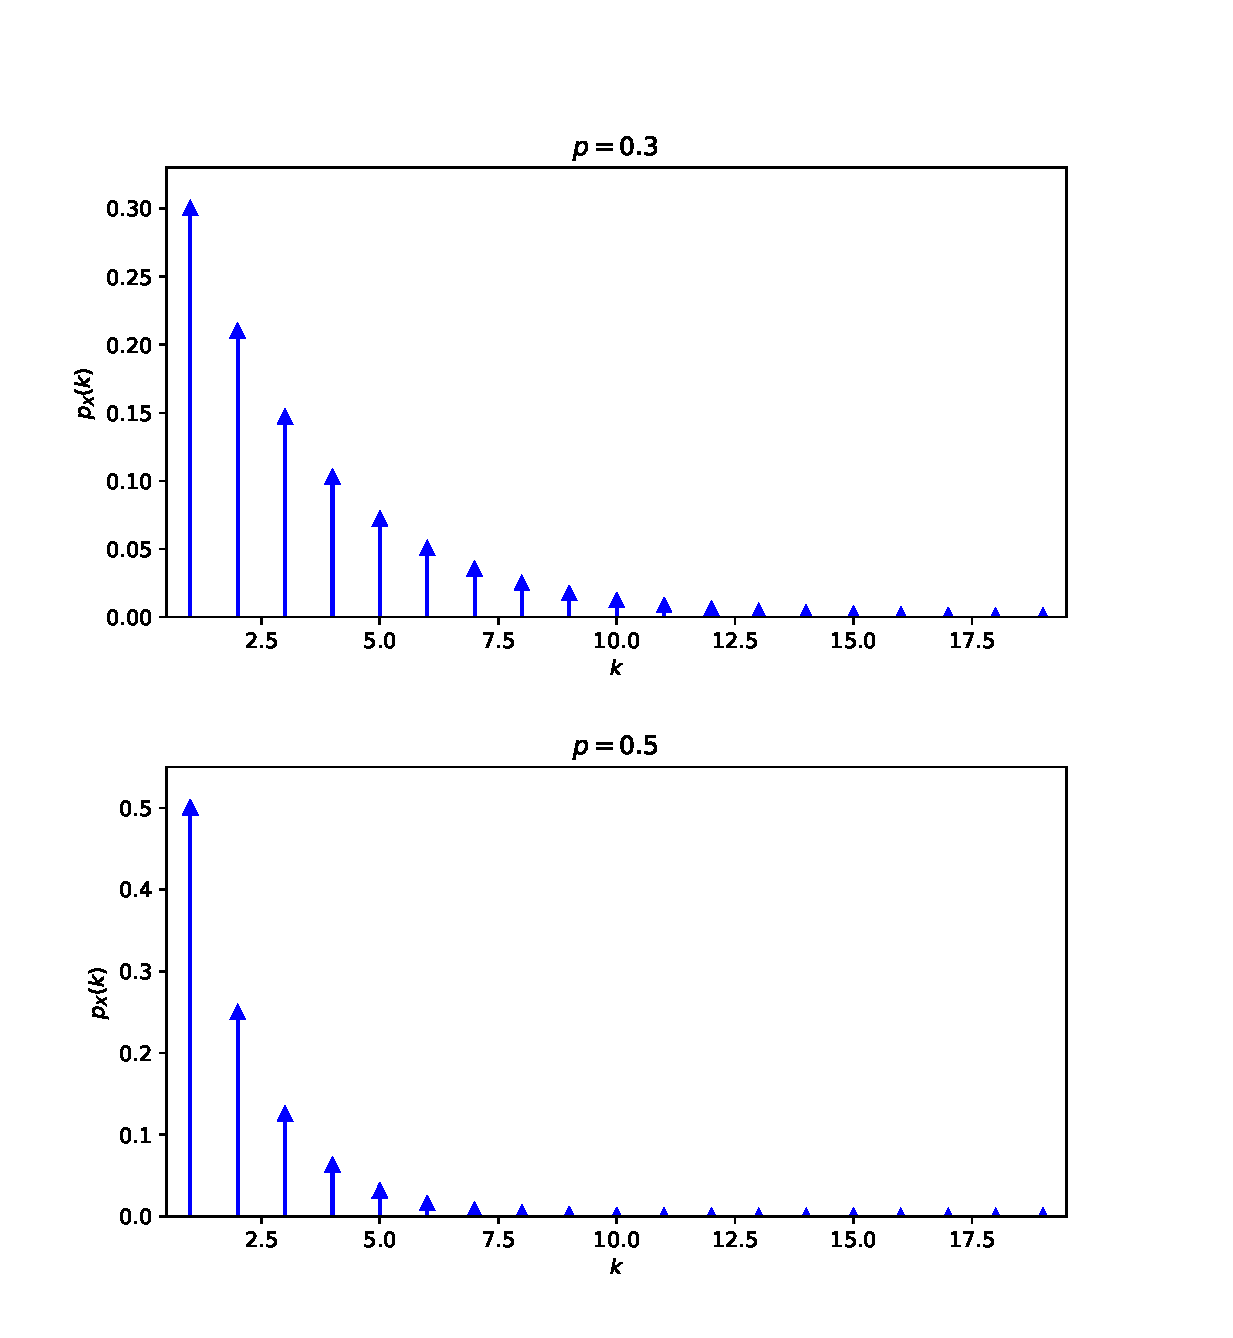
\includegraphics[width=.7\linewidth]{figures/geom_pmf}
	\caption{The PMFs of the two \geomrv s}
	\label{fig-geom-pmf}
	\end{center}\end{figure}


	\item As $p$ increases, the PMF decays more rapidly.

	\item \emph{The larger $p$ becomes, the smaller \Exp{X}\ becomes},
	which makes sense since the larger probability $p$,
	the sooner the heads comes up.

	\item The larger $p$ becomes, the smaller \VAR{X} becomes.

	\item The geometric random variable is \emph{the only discrete random variable
	that satisfies the memoryless property}:
	\beql{eq-memoryless-prop}
		\cpr{X\geq k+j}{X > j} = \pr{X\geq k}
	\eeql
	for all $j$ and $k$.
	The above expression states that
	if a success has not occurred in the first $j$ trials,
	then the probability of having to perform at least $k$ more trials
	is the same as the probability of initially having to perform at least $k$ trials.
	Thus, each time a failure occurs,
	\emph{the system ``forgets''} and begins anew
	as if it were performing the first trial.

\eit

\subsection{The Poisson Random Variables}
\bit
	\item The \possrv\ arises in situations where the events occur
	\emph{``completely at random'' in time or space}.
	For example, the Poisson random variable arises
	in counts of emissions from radioactive substances,
	in counts of demands for telephone connections,
	and in counts of defects in a semiconductor chip.

	Suppose that $\alpha$ is the average number of event occurrences
	in a specified time interval or region in space.
	Then
	\begin{itemize}
		\item range:
		\beql{eq-range-poss}
			\ssx = \{0,1,\ldots \}.
		\eeql
		\item PMF:
		\beql{eq-pmf-poss}
			\pmfxk{k} = \frac{\al^k}{k!}e^{-\al}.
		\eeql
		\figurename~\ref{fig-poss-pmf} shows the PMFs of three \possrv s;
		$\alpha=0.75$, $\alpha=3$, and $\alpha=9$.

		\item mean and variance:
		\beql{eq-mean-poss}
			\Exp{X} = \al.
		\eeql
		\beql{eq-var-poss}
			\VAR{X} = \al.
		\eeql
	\end{itemize}

	\begin{figure}\begin{center}
	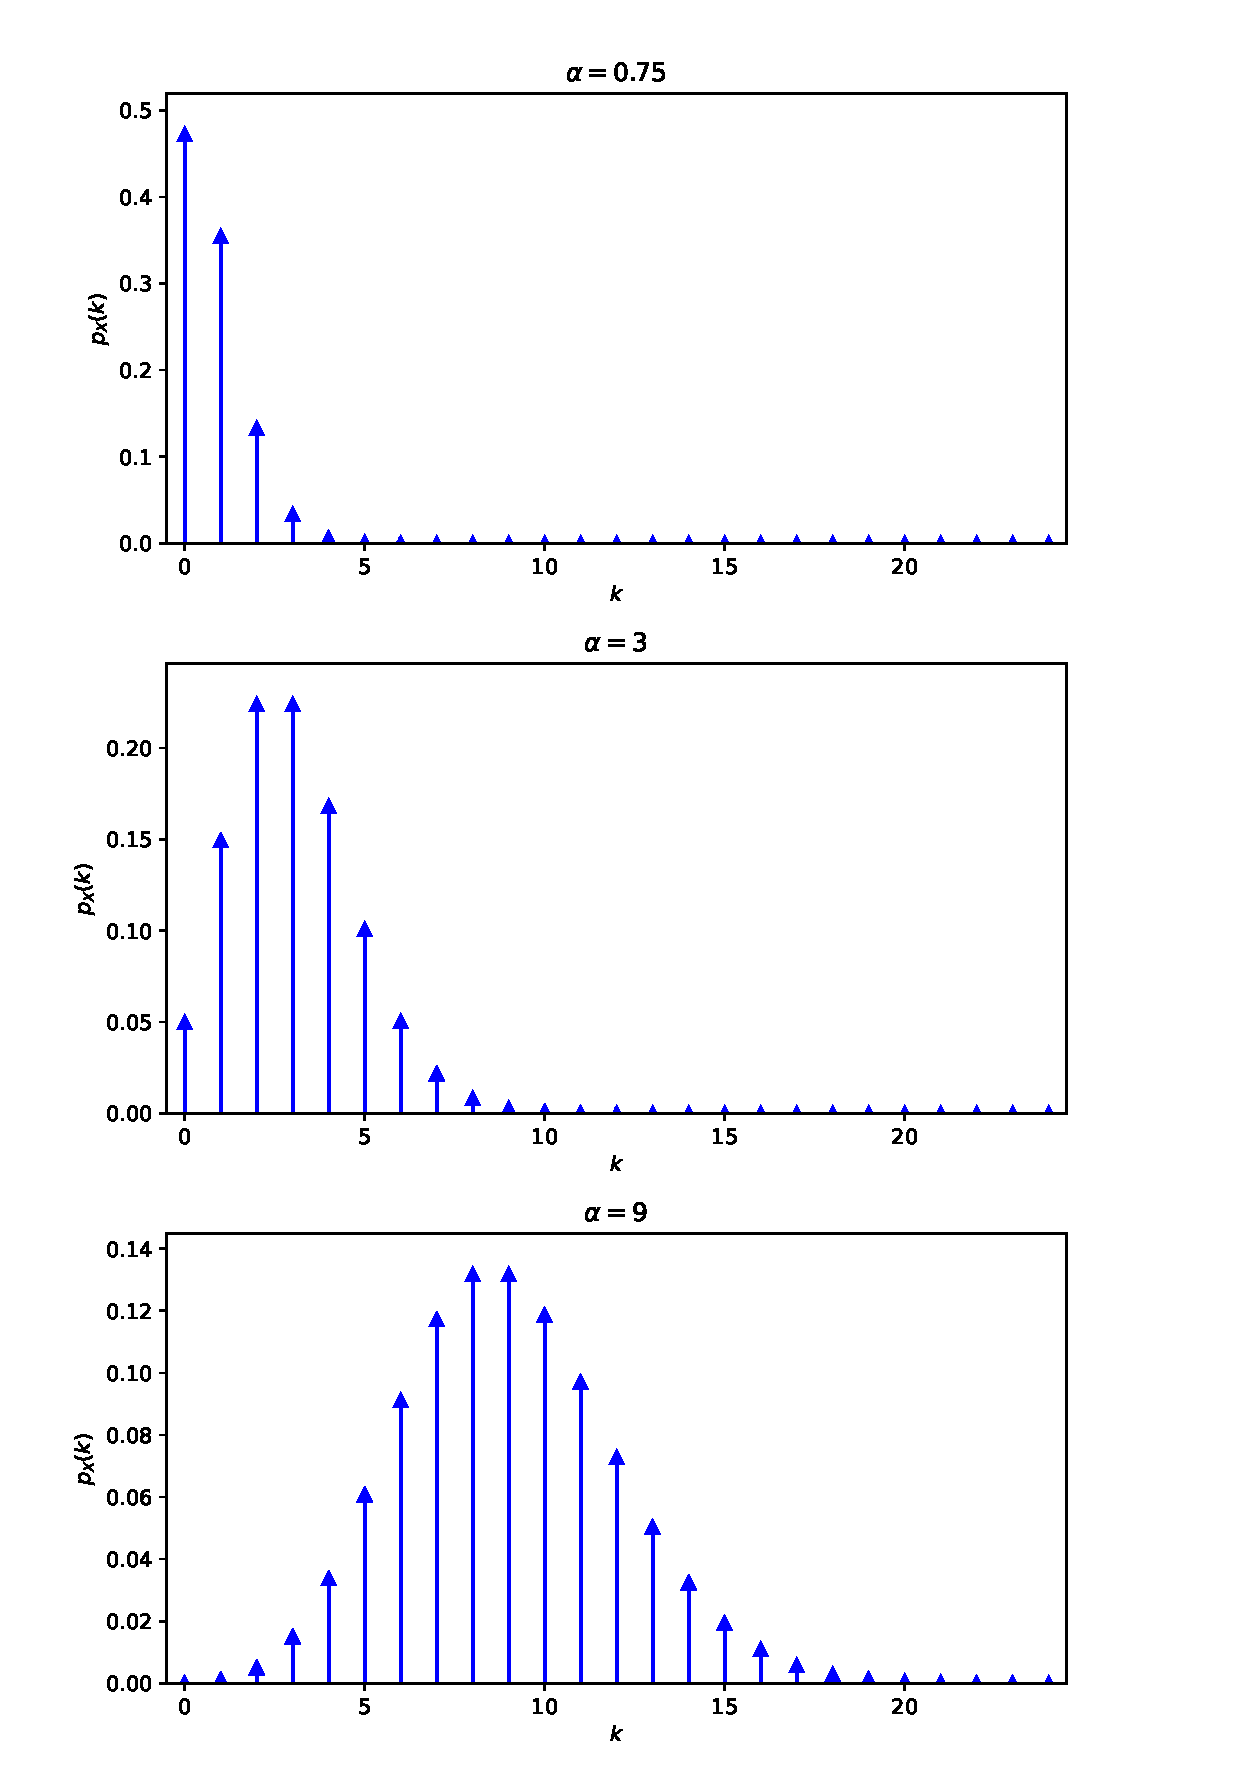
\includegraphics[width=.7\linewidth]{figures/poss_pmf}
	\caption{The PMFs of \possrv s}
	\label{fig-poss-pmf}
	\end{center}\end{figure}

	\begin{proof}
	The convergence of the Taylor's series of the exponential function
	(\ref{eq-taylor-exp})
	implies
	\[
		e^x = \sumto{k}{0}{\infty} \frac{x^k}{k!}
	\]
	for any $x\in\reals$,
	thus
	\[
		\sumkztoi \pmfxk{k}
		= \sumkztoi \frac{\al^k}{k!}e^{-\al}
		= e^{-\al} \sumkztoi \frac{\al^k}{k!}
		= 1.
	\]
	Then the expected value is
	\[
		\Exp{X}
		= \sumkztoi k \pmfxk{k}
		= \sumktoi k \frac{\al^k}{k!}e^{-\al}
		= \al \sumktoi \frac{\al^{k-1}}{(k-1)!}e^{-\al}
		= \al
	\]
	also by (\ref{eq-taylor-exp}).
	The second moment of \X\ is
	\begin{eqnarray*}
		\lefteqn{
		\Exp{X^2}
		= \sumktoi k^2 \pmfxk{k}
		= \sumktoi k \frac{\al^k}{(k-1)!}e^{-\al}
		= \sumktoi ((k-1)+1) \frac{\al^k}{(k-1)!}e^{-\al}
		}
		\\&=&
		 \sumto{k}{2}{\infty} \frac{\al^k}{(k-2)!}e^{-\al}
		+ \sumktoi \frac{\al^k}{(k-1)!}e^{-\al}
		\\&=&
		\al^2 \sumto{k}{2}{\infty} \frac{\al^{k-2}}{(k-2)!}e^{-\al}
		+ \al \sumktoi \frac{\al^{k-1}}{(k-1)!}e^{-\al}
		\\&=&
		\al^2 + \al,
	\end{eqnarray*}
	hence
	\[
		\VAR{X} = \Exp{X^2} - \Exp{X}^2 = \al.
	\]
	\qed

	\end{proof}


	\item For $\al < 1$, \pmfxk{k}\ is maximum at $k = 0$;
	for $\al > 1$, \pmfxk{k}\ is maximum at \floor{\al};
	if \al\ is a positive integer,
	the \pmfxk{k}\ is maximum at $k = \al$ and at $k = \al - 1$.

	\item \lgexam{3.30}{Queries at a Call Center}
	The number $N$ of queries arriving in $t$ seconds at a call center
	is a Poisson random variable with $\al = \ld t$ where \ld\
	is the average arrival rate in queries/second.
	Assume that the arrival rate is four queries per minute.
	Find the probability of the following events:
	(a) more than $4$ queries in $10$ seconds;
	(b) fewer than $5$ queries in $2$ minutes.

	In part (a), the average number of queries for $10$ seconds is $\al=4/6=2/3$.
	Thus, the probability that more than $4$ queries arrive in $10$ seconds
	is
	\[
		\pr{X>4} = 1- \pr{X\leq 4} = 1-\sumto{k}{0}{4} \posspmf{(2/3)}{k}
		= 6.33 \times 10^{-4}.
	\]
	In part (b), the average number of queries for $2$ minutes is $\al=4\cdot 2=8$.
	Thus, the probability that fewer than $5$ queries arrive in $2$ minutes
	is
	\[
		\pr{X<5} = \sumto{k}{0}{4} \posspmf{8}{k} = 0.996.
	\]
	These values were obtained by the following python code.
\begin{verbatim}
>>> import scipy.stats as ss
>>> rv = ss.poisson(2/3.)
>>> 1-rv.cdf(4)
0.00063252138923441947
>>> rv = ss.poisson(8.)
>>> rv.cdf(4)
0.099632400487045969
>>>
\end{verbatim}

	\item
	One of the applications of the Poisson probabilities in
	(\ref{eq-pmf-poss}) is
	to \emph{approximate the binomial probabilities in the case where $p$ is very small
	and $n$ is very large},
	that is,
	where the event $A$ of interest is very rare
	but the number of Bernoulli trials is very large.
	If $\al = np$ is fixed, then as $n$ becomes large:
	\beql{eq-binom-conv-poss}
		\lim_{n\to\infty} \binompmf{n}{p}{k} = \posspmf{\al}{k}
	\eeql
	for $k=0,1,\ldots$.
	\begin{proof}
	If we let $\al=np$,
	\begin{eqnarray*}
		\lefteqn{
			\dbinompmf
			= \frac{n(n-1)\cdots (n-k+1)}{k!} p^k (1-p)^{n-k}
		}
		\\&=&
		\frac{(1-p)^{-k}}{k!}
		n(n-1)\cdots (n-k+1) p^k (1-p)^n
		\\&=&
		\frac{(1-p)^{-k}}{k!}
		(np)(np-p)\cdots (np-(k-1)p) (1-\al/n)^{n}
		\\&=&
		\frac{(1-p)^{-k}}{k!}
		(\al)(\al-p)\cdots (\al-(k-1)p) (1-\al/n)^{n}.
	\end{eqnarray*}
	Now if we fix $\al=np$ and let $n$ go to $\infty$,
	$p$ goes to $0$,
	hence
	\[
		\lim_{n \to \infty} \dbinompmf = \frac{\al^k }{k!} e^{-\al}
	\]
	where
	we use
	\[
		\lim_{n\to\infty} (1-\al/n)^n
		= \lim_{n\to\infty} (1+1/n)^{-\al n}
		= \left( \lim_{n\to\infty} (1+1/n)^n \right)^{-\al}
		= e^{-\al}.
	\]


	\end{proof}

	\item
	The Poisson random variable appears
	in numerous physical situations
	because many models are very large in scale and involve very rare events.
	\begin{itemize}
		\item
		For example,
		the Poisson PMF gives an accurate prediction
		for the relative frequencies of the number of particles emitted
		by a radioactive mass during a fixed time period.
		This correspondence can be explained as follows.
		A radioactive mass is composed of a large number of atoms,
		say $n$.
		In a fixed time interval each atom has a very small probability $p$
		of disintegrating and emitting a radioactive particle.
		If atoms disintegrate independently of other atoms,
		then the number of emissions in a time interval
		can be viewed as the number of successes in $n$ trials.
		For example, one microgram of radium contains about $n = 10^{16}$ atoms,
		and the probability that a single atom will disintegrate
		during a one-millisecond time interval is $p = 10^{-15}$ [Rozanov, p. 58]. 
		Thus it is an understatement to say that the conditions
		for the approximation in (\ref{eq-binom-conv-poss}) hold:
		$n$ is so large and $p$ so small that one could argue
		that the limit $n \to \infty$ has been carried out
		and that the number of emissions is \emph{exactly}
		a \possrv.
	\end{itemize}
	
\eit

\subsection{The Uniform Random Variable}

\bit
	\item
	The discrete uniform random variable $X$ takes on values
	in a set of consecutive integers $\ssx = \{j + 1, \ldots, j + L\}$
	with equal probability:
	\begin{itemize}
		\item range:
		\beql{eq-range-disc-unif}
			\ssx = \{j+1,j+2,\ldots,j+L \}.
		\eeql
		\item PMF:
		\beql{eq-pmf-disc-unif}
			\pmfxk{k} = \frac{1}{L}.
		\eeql

		\item mean and variance:
		\beql{eq-mean-disc-unif}
			\Exp{X} = j + \frac{L+1}{2}.
		\eeql
		\beql{eq-var-disc-unif}
			\VAR{X} = \frac{L^2-1}{12}.
		\eeql
	\end{itemize}

	\item
	This humble random variable occurs
	whenever outcomes are equally likely, \eg,
	toss of a fair coin or a fair die,
	spinning of an arrow in a wheel divided into equal segments,
	selection of numbers from an urn.
\eit

\subsection{The Zipf Random Variable}

\bit
	\item
	The Zipf \randvar\ is named for
	George Zipf who observed that the frequency of words
	in a large body of text is proportional to their rank.
	Suppose that words are ranked from most frequent,
	to next most frequent, and so on.
	Let \X\ be the rank of a word,
	then $\ssx = \{1, 2, ..., L\}$
	where $L$ is the number of distinct words.
	\begin{itemize}
		\item range:
		\beql{eq-range-zipf}
			\ssx = \{1,2,\ldots,L\}.
		\eeql
		\item PMF:
		\beql{eq-pmf-zipf}
			\pmfxk{k} = \frac{1}{c_L} \frac{1}{k}.
		\eeql
		where $c_L$ is a normalization constant:
		\beql{eq-zipf-norm-const}
			c_L = \sumto{j}{1}{L} = 1 + \frac{1}{2} + \frac{1}{3} + \cdots + \frac{1}{L}.
		\eeql

		\item mean and variance:
		\beql{eq-mean-zipf}
			\Exp{X} = \frac{L}{c_L}.
		\eeql
		\beql{eq-var-zipf}
			\VAR{X} = \frac{L(L+1)}{2c_L} - \frac{L^2}{c_L^2}.
		\eeql
	\end{itemize}

	\item
	The constant $c_L$ occurs frequently in calculus
	and is called the $L$th harmonic mean
	and increases approximately as $\log L$.
	For example, for $L = 100$, $c_L = 5.187378$
	and $c_L - \log L = 0.582207$.
	It can be shown that as $L \to \infty$,
	$c_L - \log L \to 0.57721$.

	\item
	The Zipf and related random variables
	have gained prominence with the growth of the Internet
	where they have been found in a variety of measurement studies
	involving Web page sizes,
	Web access behavior, and Web page interconnectivity.
	These random variables had previously been found extensively
	in studies on the distribution of wealth and,
	not surprisingly, are now found in Internet video rentals and book sales.
\eit

\section{Generation of Discrete Random Variables}

MAYBE LATER WITH OTHER RELATED TOPICS


